\input{def/preambule}
\begin{document}
	%%%%%%%%%%%%%%%
	%% RENEWCOMMAND
	%%%%%%%%%%%%%%%
	\renewcommand\labelitemi{\textbullet}
	\renewcommand\labelitemii{$\circ$}
	\renewcommand\labelitemiii{$\star$}
	% redefines the itemizing symbols for the itemize environment, 
	% cannot redefine the 4th lvl, 
	% cannot have more than 4 lvls,
	% in french, by default, it's all dashes...
	
	%%%%%%%%%%%%%
	%% TITLE PAGE
	%%%%%%%%%%%%%
	\hypersetup{pageanchor=false}
\begin{titlepage}
	
	\begin{center} 
		\includegraphics[height=0.8cm]{logo_epfl} 
	\end{center}
	
	\vfill
	
	\begin{center}
		\rule{\linewidth}{1mm}
		\bigskip
		
		\Huge \title\\
		\bigskip
		
		\Large \subtitle\\
		\bigskip
		
		\rule{1cm}{0.3mm}\\
		\bigskip		
		
		\large \students\\
		\bigskip
		
		\date
		\bigskip
		
		\rule{\linewidth}{1mm}
		\vfill

		\small \division

		\vfill
		
		\small{
			\begin{tabular}{l@{: }l}
				Professor &\professor\\
				Last update &\today\\
				Place &\place\\
				SCIPERs &\sciper\\
			\end{tabular} 
		}
	\end{center} 
\end{titlepage}
\hypersetup{pageanchor=true}
\newpage
	
	%%%%%%%%%%%%%%%%%%%
	%% TABLE OF CONTENT
	%%%%%%%%%%%%%%%%%%%
	\setcounter{page}{1} % beginning of page numeration here
	\tableofcontents
	\newpage
	
	%%%%%%%%
	%% INPUT
	%%%%%%%%
	\section{Introduction}

The objective of this assignment is to construct metrics and find optimal parameters for the controller, using testing weights and an objective speed. We chose to give the same weight to the effort and the target speed, as nothing contrary to this was indicated, and we settled for a target speed of $0.7$ since the observed mean speed for the initial parameters was around $0.4$.

	\section{Methods}

\subsection{Modelization}

In engineering at large (not just robotics), the idea of modelization is to abstract the (real physical) system of interest into a mathematical object that can be used, calculated upon, simulated upon.
Examples include modelizing the working of motor by an electrical circuit; modelizing the working of a pump by a fluid circuit; modelizing a plant by control system, etc$\dots$
The benefits are two-fold: the process of modelizing forces the engineer to understand the system, and what of the system is relevant to the engineer's research; and upon completion, it also allows the engineer to apply mathematical tools to its system, like control design, simulation, etc$\dots$

\vspace{\baselineskip}

In the field of robotics, modelization's end product are the kinematics and dynamics of the robot.
That modelization doesn't have to be done from scratch, because tools are at disposal, that help both in modelizing the robot, and in unifying its representation (like the urdf, for example).
Nonetheless, for this project, the modelization is done from scratch for academic value.

\vspace{\baselineskip}

The starting point is the Figure~\ref*{fig::model}, because in our case, there is no real robot, it was just decided to work on a generic three-link 2D biped model.

\subsubsection{Kinematics}

% generate kinematics.mlx
% visualize.m

The kinematics of the robot consist in the equations for the positions $\mathbf{x}_i = \begin{pmatrix}
	x_i \\ z_i
\end{pmatrix}$ of the robot links and their respective velocities $\text{d}\mathbf{x}_i$ expressed in relation to the generalized coordinates $\mathbf{q} = \begin{bmatrix}
q_1 \\ q_2 \\ q_3
\end{bmatrix}$ and their derivative $\text{d}\mathbf{q}$:

\begin{align*}
	x_1 &= \dfrac{l_{1}\,\sin\left(q_{1}\right)}{2} \\
	x_2 &= l_{1}\,\sin\left(q_{1}\right)-\dfrac{l_{2}\,\sin\left(q_{2}\right)}{2} \\
	x_3 &= l_{1}\,\sin\left(q_{1}\right)+\dfrac{l_{3}\,\sin\left(q_{3}\right)}{2} \\
	z_1 &= \dfrac{l_{1}\,\cos\left(q_{1}\right)}{2} \\
	z_2 &= l_{1}\,\cos\left(q_{1}\right)-\dfrac{l_{2}\,\cos\left(q_{2}\right)}{2} \\
	z_3 &= l_{1}\,\cos\left(q_{1}\right)+\dfrac{l_{3}\,\cos\left(q_{3}\right)}{2} \\
	\text{d}x_1 &= \dfrac{\mathrm{dq}_{1}\,l_{1}\,\cos\left(q_{1}\right)}{2} \\
	\text{d}x_2 &= \mathrm{dq}_{1}\,l_{1}\,\cos\left(q_{1}\right)-\dfrac{\mathrm{dq}_{2}\,l_{2}\,\cos\left(q_{2}\right)}{2} \\
	\text{d}x_3 &= \mathrm{dq}_{1}\,l_{1}\,\cos\left(q_{1}\right)+\dfrac{\mathrm{dq}_{3}\,l_{3}\,\cos\left(q_{3}\right)}{2} \\
	\text{d}z_1 &= -\dfrac{\mathrm{dq}_{1}\,l_{1}\,\sin\left(q_{1}\right)}{2} \\
	\text{d}z_2 &= \dfrac{\mathrm{dq}_{2}\,l_{2}\,\sin\left(q_{2}\right)}{2}-\mathrm{dq}_{1}\,l_{1}\,\sin\left(q_{1}\right) \\
	\text{d}z_3 &= -\mathrm{dq}_{1}\,l_{1}\,\sin\left(q_{1}\right)-\dfrac{\mathrm{dq}_{3}\,l_{3}\,\sin\left(q_{3}\right)}{2}
\end{align*}

\subsubsection{Dynamics}

% generate dynamics.mlx
% eval M.m, eval C.m, eval G.m, eval B.m

Computing the dynamics means computing the mass matrix $\mathbf{M}$, Coriolis matrix $\mathbf{C}$, gravity matrix $\mathbf{G}$ and control matrix $\mathbf{B}$ for the robot, from the kinematics, using the Lagrangian method.
This allows to have the equation of motion for the robot:

\begin{align*}
	\mathbf{M}\left(\mathbf{q}\right)\mathbf{\ddot{q}} + \mathbf{C}\left(\mathbf{q},\mathbf{\dot{q}}\right)\mathbf{\dot{q}} + \mathbf{G}\left(\mathbf{q}\right) &= \mathbf{Bu}
\end{align*}

The first step is to compute the Langrangian of the system:

\begin{align*}
	\underbrace{L}_\text{Lagrangian} &= \underbrace{T}_\text{total kinetic energy} - \underbrace{V}_\text{total potential energy} \\
	&= \left(T_1+T_2+T_3\right) - \left(V_1+V_2+V_3\right) \\
	&= \sum_{i=1}^{3} \dfrac{1}{2} m_i \mathbf{\dot{x}}^2 - \sum_{i=1}^{3} m_i g z_i \\
\end{align*}

with $i$ denoting the links of the robot.

\vspace{\baselineskip}

The Lagrange equation states that:

\begin{equation*}
	\dfrac{\text{d}}{\text{d}t}\left(\dfrac{\partial L}{\partial \dot{q}_i}\right) = \dfrac{\partial L}{\partial q_i}
\end{equation*}

From this last equation, the matrices $\mathbf{M}$, $\mathbf{C}$ and $\mathbf{G}$ are deduced by substitution.
To verify that the substitution is correct, the error on the following is computed (and the error should amount to zero, obviously):

\begin{equation*}
	\left( \mathbf{M}\left(\mathbf{q}\right)\mathbf{\ddot{q}} + \mathbf{C}\left(\mathbf{q},\mathbf{\dot{q}}\right)\mathbf{\dot{q}} + \mathbf{G}\left(\mathbf{q}\right) \right) - \left( \dfrac{\text{d}}{\text{d}t}\left(\dfrac{\partial L}{\partial \dot{q}_i}\right) - \dfrac{\partial L}{\partial q_i}
	\right)
\end{equation*}

Then, the control matrix $\mathbf{B}$ is computed. The robot is commanded through $\mathbf{u}_1$ and $\mathbf{u}_2$ as described on Figure~\ref*{fig::model_with_command} below:

\begin{figure}[H]
	\begin{center}
		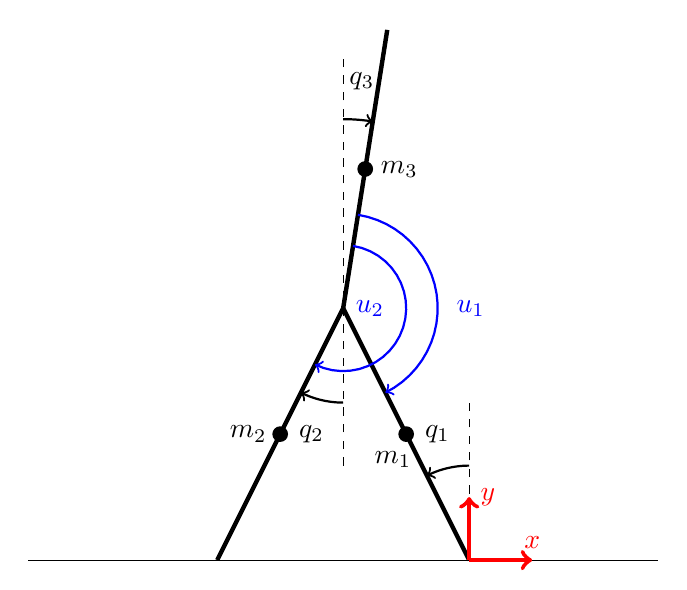
\begin{tikzpicture}
			\begin{scope}[x={8cm},y={8cm}]
				% l = 0,447213
				% alpha = 8.999999999478607 deg
				% =0.5+sqrt(0.2^2+0.4^2)*sin(pi/20)
				% =0.4+sqrt(0.2^2+0.4^2)*cos(pi/20)

				\draw[-] (0,0)--(1,0); % ground

				\draw[-,ultra thick] (0.3,0)--(0.5,0.4); % link 2
				\draw[-,ultra thick] (0.7,0)--(0.5,0.4); % link 1
				\draw[-,ultra thick] (0.5,0.4)--(0.5699596195707541,0.8417076540309386); % link 3

				\draw[dashed] (0.5,0.15)--(0.5,0.8); % big vertical dashed line
				\draw[dashed] (0.7,0)--(0.7,0.25); % small vertical dashed line

				\draw[->,ultra thick, red] (0.7,0)--(0.8,0) node[above]{$x$}; % x axis
				\draw[->,ultra thick, red] (0.7,0)--(0.7,0.1) node[right]{$y$}; % y axis

				\draw [->,thick,domain=81.00000000052139:-63.4349488, blue] plot ({0.5+0.15*cos(\x)}, {0.4+0.15*sin(\x)}); % u1
				\draw [->,thick,domain=81.00000000052139:-116.5650512, blue] plot ({0.5+0.10*cos(\x)}, {0.4+0.10*sin(\x)}); % u2

				\draw [->,thick,domain=-90:-116.5650512] plot ({0.5+0.15*cos(\x)}, {0.4+0.15*sin(\x)}); % q2
				\draw [->,thick,domain=90:116.5650512] plot ({0.7+0.15*cos(\x)}, {0.15*sin(\x)}); % q1
				\draw [->,thick,domain=90:81.00000000052139] plot ({0.5+0.3*cos(\x)}, {0.4+0.3*sin(\x)}); % q3

				\node at (0.4,0.2) [circle,fill,inner sep=1]{.}; % m2
				\node at (0.6,0.2) [circle,fill,inner sep=1]{.}; % m1
				\node at (0.5349798097853771,0.6208538270154693) [circle,fill,inner sep=1]{.}; % m3

				\node[text width=0mm] at (0.63,0.2) {$q_1$};
				\node[text width=0mm] at (0.43,0.2) {$q_2$};
				\node[text width=0mm] at (0.51,0.76) {$q_3$};

				\node[text width=0mm] at (0.55,0.16) {$m_1$};
				\node[text width=0mm] at (0.32,0.2) {$m_2$};
				\node[text width=0mm] at (0.56,0.62) {$m_3$};

				\node[text width=0mm, blue] at (0.68,0.4) {$u_1$};
				\node[text width=0mm, blue] at (0.52,0.4) {$u_2$};
			\end{scope}
		\end{tikzpicture}
	\end{center}
	\caption{Representation of the three-link 2D biped model with the angle commands.}
	\label{fig::model_with_command}
\end{figure}

This means that the model is underactuated, because there is more DOFs than actuated joints.

\vspace{\baselineskip}

The work done by $\mathbf{u}_1$ and $\mathbf{u}_2$ is computed as the product of $\mathbf{u}_i$ and the corresponding virtual angle variation.
Then, the control matrix is computed by substitution.

\vspace{\baselineskip}

The obtained matrices are:

\begin{align*}
	\mathbf{M} &= \begin{bmatrix}
		{l_{1}}^2\,\left(\dfrac{m_{1}}{4}+m_{2}+m_{3}\right) & -\dfrac{l_{1}\,l_{2}\,m_{2}\,\cos\left(q_{1}-q_{2}\right)}{2} & \dfrac{l_{1}\,l_{3}\,m_{3}\,\cos\left(q_{1}-q_{3}\right)}{2}\\ -\dfrac{l_{1}\,l_{2}\,m_{2}\,\cos\left(q_{1}-q_{2}\right)}{2} & \dfrac{{l_{2}}^2\,m_{2}}{4} & 0\\ \dfrac{l_{1}\,l_{3}\,m_{3}\,\cos\left(q_{1}-q_{3}\right)}{2} & 0 & \dfrac{{l_{3}}^2\,m_{3}}{4}
	\end{bmatrix} \\
	\mathbf{C} &= \begin{bmatrix}
		0 & -\dfrac{\mathrm{dq}_{2}\,l_{1}\,l_{2}\,m_{2}\,\sin\left(q_{1}-q_{2}\right)}{2} & \dfrac{\mathrm{dq}_{3}\,l_{1}\,l_{3}\,m_{3}\,\sin\left(q_{1}-q_{3}\right)}{2}\\ \dfrac{\mathrm{dq}_{1}\,l_{1}\,l_{2}\,m_{2}\,\sin\left(q_{1}-q_{2}\right)}{2} & 0 & 0\\ -\dfrac{\mathrm{dq}_{1}\,l_{1}\,l_{3}\,m_{3}\,\sin\left(q_{1}-q_{3}\right)}{2} & 0 & 0
	\end{bmatrix} \\
	\mathbf{G} &= \begin{bmatrix}
		-\dfrac{g\,l_{1}\,\sin\left(q_{1}\right)\,\left(m_{1}+2\,m_{2}+2\,m_{3}\right)}{2}\\ \dfrac{g\,l_{2}\,m_{2}\,\sin\left(q_{2}\right)}{2}\\ -\dfrac{g\,l_{3}\,m_{3}\,\sin\left(q_{3}\right)}{2}
	\end{bmatrix} \\
	\mathbf{B} &= \begin{bmatrix}
		1 & 0\\ 0 & 1\\ -1 & -1
	\end{bmatrix}
\end{align*}

It is interesting to notice that the mass matrix $\mathbf{M}$ corresponds to the Jacobian of the total kinetic energy $T$ with respect to the generalized coordinates.
That is a normal result, since kinetic energy is derived from moving masses.% (\textbf{assignement 1 question}).

\subsubsection{Impact map}

% generate impact map.mlx (in the “generate model” folder)
% eval A m.m, eval A p.m (in the “dynamics” folder)
% impact.m (in the “dynamics” folder)

In the hybrid model of walking, the model oscillates between the single support swing phase and the impact phase, during which the leg roles are switched, like so:

\begin{center}
	\begin{tikzpicture}[auto]
		\node [block] (swing) {Single support swing phase};
		\node [block, right=of swing] (impact) {Impact phase};

		\draw [->] (swing) |- (0, 1.5) -| (impact);
		\draw [<-] (swing) |- (0, -1.5) -| (impact);
	\end{tikzpicture}
\end{center}

The modelization of the swing phase has been extensively described in the previous sections, leading to the kinematics and dynamics of the robot during the single support swing phase through the Lagrangian method.

\vspace{\baselineskip}

This section is concerned with the impact phase.
This phase is based on the assumptions that:

\begin{itemize}
	\item the impact and leg role switching is instantaneous and
	\item the support leg does not slip.
\end{itemize}

Because of the assumption of instantaneousness, there is no need for (and it would prove to be quite difficult to) develop kinematics and dynamics for the impact phase.
Instead, the state of the robot is mapped from right before the impact to right after the impact, throught the use of the impact map $\mathbf{\Delta}$ computed by conservation of the angular momentum.
In particular, we can write:

\begin{align*}
	\mathbf{\Delta} \left( \mathbf{q}_m, \mathbf{\dot{q}}_m \right) &= \begin{bmatrix}
		\mathbf{\Delta}_q \left( \mathbf{q}_m \right) &  \mathbf{\Delta}_{\dot{q}} \left( \mathbf{q}_m, \mathbf{\dot{q}}_m \right)
	\end{bmatrix}
\end{align*}

The angular positions are the same (semantically) before and after impact, so the mapping only needs to account for the change of reference frame.

\vspace{\baselineskip}

On the contrary, the angular velocities after impact are computed using the McGeer method~\cite{mcgeer}, which is a conservation of angular momentum method: the angular momentum before impact $H_m$ must be equal to the angular momentum after impact $H_p$:

\begin{align*}
	H_m &= H_p \\
	A_m\mathbf{\dot{q}}_m &= A_p\mathbf{\dot{q}}_p \\
	\mathbf{\dot{q}}_p &= A_{p}^{-1}A_m\mathbf{\dot{q}}_m
\end{align*}

After computation:

\tiny

\begin{align*}
	A_p &= \begin{bmatrix}
		\dfrac{l_{1}\,l_{2}\,m\,\cos\left(q_{1,p}-q_{2,p}\right)}{2}-{l_{1}}^2\,m_{3}-\dfrac{5\,{l_{1}}^2\,m}{4}-\dfrac{l_{1}\,l_{3}\,m_{3}\,\cos\left(q_{1,p}-q_{3,p}\right)}{2} & \dfrac{l_{1}\,l_{2}\,m\,\cos\left(q_{1,p}-q_{2,p}\right)}{2}-\dfrac{{l_{2}}^2\,m}{4} & -\dfrac{m_{3}\,{l_{3}}^2}{4}-\dfrac{l_{1}\,m_{3}\,\cos\left(q_{1,p}-q_{3,p}\right)\,l_{3}}{2}\\ \dfrac{l_{1}\,l_{2}\,m_{3}\,\cos\left(q_{1,p}-q_{2,p}\right)}{2} & -\dfrac{{l_{2}}^2\,m_{3}}{4} & 0\\ -\dfrac{l_{1}\,l_{3}\,m\,\cos\left(q_{1,p}-q_{3,p}\right)}{2} & 0 & -\dfrac{{l_{3}}^2\,m}{4}
	\end{bmatrix} \\
	A_m &= \begin{bmatrix}
		\dfrac{{l_{1}}^2\,m}{4}-l_{1}\,l_{2}\,m\,\cos\left(q_{1,m}-q_{2,m}\right)-l_{1}\,l_{2}\,m_{3}\,\cos\left(q_{1,m}-q_{2,m}\right)-\dfrac{l_{1}\,l_{3}\,m_{3}\,\cos\left(q_{1,m}-q_{3,m}\right)}{2} & \dfrac{{l_{2}}^2\,m}{4} & -\dfrac{m_{3}\,{l_{3}}^2}{4}-\dfrac{l_{2}\,m_{3}\,\cos\left(q_{2,m}-q_{3,m}\right)\,l_{3}}{2}\\ \dfrac{{l_{1}}^2\,m_{3}}{4} & 0 & 0\\ -\dfrac{l_{1}\,l_{3}\,m\,\cos\left(q_{1,m}-q_{3,m}\right)}{2} & 0 & -\dfrac{{l_{3}}^2\,m}{4}
	\end{bmatrix}
\end{align*}

\normalsize

with $m=m_1=m_2$, and thus both $\mathbf{q}_p$ and $\mathbf{\dot{q}}_p$ can be computed.

\vspace{\baselineskip}

\textbf{Assignement 2 questions:}

\begin{enumerate}
	\item \textit{What can you say about the potential energy before and after impact?}
	
	The potential energy before and after the impact are the same, since the frame of reference is moved from one foot to another without any change in the position, velocity or acceleration of the different masses.
	\item \textit{Try $\mathbf{q}_m = \begin{bmatrix}
		pi/6 & -pi/6 & pi/10
	\end{bmatrix}$, $\mathbf{\dot{q}}_m = \begin{bmatrix}
		1 & 0.2 & 0
	\end{bmatrix}$. What percentage of the kinetic energy of the biped is lost due to the impact?}

	Computing using our functions, we find that 38.73\% of the kinetic energy is lost during the impact of the foot for those parameters.
	\item \textit{Plot the percentage of the kinetic energy loss due to impact as a function of angle $\alpha$ where $\mathbf{q}_m=\begin{bmatrix}
		\alpha & -\alpha & 0
	\end{bmatrix}$ and $\alpha$ varies from 0 to $\pi/4$. Assume that $\mathbf{\dot{q}} = \begin{bmatrix}
		1 & 0.2 & 0
	\end{bmatrix}$.}

	\begin{figure}[H]
		\begin{center}
			\includegraphics[angle=0,width=0.7\textwidth]{kinetic_energy_loss_along_leg_angle}
		\end{center}
		\caption{Percentage of kinetic energy loss as a function of leg angle.}
	\end{figure}
	\item \textit{The bigger $\alpha$ is, the bigger is the step length. Based on your answer to question 3, what is the relation between step length and energy loss at impact given a fixed $\mathbf{\dot{q}}_m$?}
	
	The energy loss appears to be akin to a square root function. The bigger the step, the bigger the energy loss : if there is no step at all (i.e. if $\alpha=0$), there is no energy loss. If we were to optimize the energy loss over the distance travelled, we'd have to look for the inflexion point (which is approximately at $\alpha = \SI{0.15}{\radian}$), because the energy loss increases slowlier at first (from $\alpha=0$ to $\alpha\sim\SI{0.15}{\radian}$), and then faster.  
\end{enumerate}

	\section{Results}

\subsection{Virtual constraints controller}

When optimizing on the objective function~\ref{eq::virtual_constraints_objective_fun} with $w_1 = w_2 = 0.5$, and $\dot{x} = \SI{0.7}{\meter\per\second}$, the following set of optimized parameters were computed:

\begin{align*}
	\mathbf{q}_0 &= \begin{bmatrix}
		0.3239 \\ -0.3496 \\ \num{3.746e-4}
	\end{bmatrix} \\
	\mathbf{\dot{q}}_0 &= \begin{bmatrix}
		\num{2.894e-04} \\ \num{1.720e-04} \\ 8.583
	\end{bmatrix} \\
	k_{p1} &= 452.6 \\
	k_{p2} &= 102.1 \\
	k_{d1} &= 95.15 \\
	k_{d2} &= 4.619 \\
	\alpha &= 0.1911
\end{align*}

\begin{figure}[H]
	\begin{subfigure}[h]{0.495\textwidth}
		\begin{center}
			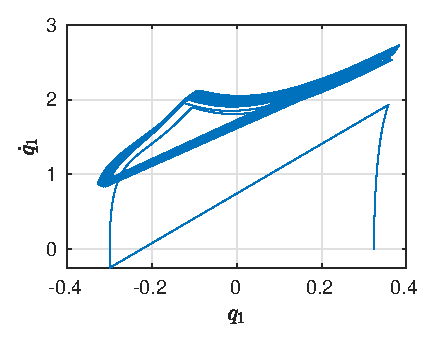
\includegraphics[width=\textwidth]{a04_state_space_q1_optimized}
			\caption{$q_1$ state-space plot}
%			\label{fig::img1}
		\end{center}
	\end{subfigure}
	\begin{subfigure}[h]{0.495\textwidth}
		\begin{center}
			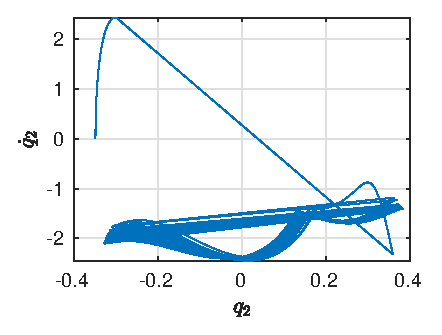
\includegraphics[width=\textwidth]{a04_state_space_q2_optimized}
			\caption{$q_1$ state-space plot}
%			\label{fig::img2}
		\end{center}
	\end{subfigure}

	\begin{subfigure}[h]{0.495\textwidth}
		\begin{center}
			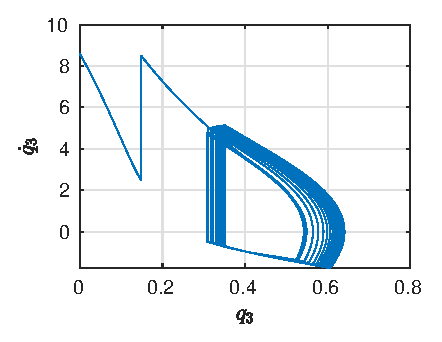
\includegraphics[width=\textwidth]{a04_state_space_q3_optimized}
			\caption{$q_1$ state-space plot}
%			\label{fig::img3}
		\end{center}
	\end{subfigure}
	\caption{State-space plot for the three generalized coordinates.}
%	\label{img::global_label}
\end{figure}

\begin{figure}[H]
	\begin{subfigure}[h]{0.495\textwidth}
		\begin{center}
			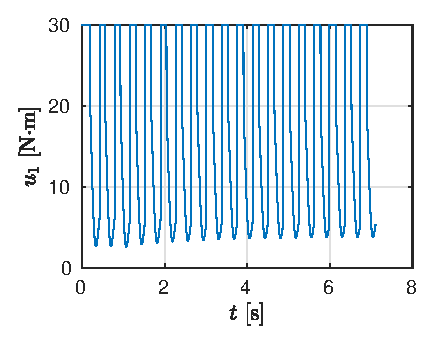
\includegraphics[width=\textwidth]{a04_control_torques_u1_optimized}
			\caption{first actuator}
		\end{center}
	\end{subfigure}
	\begin{subfigure}[h]{0.495\textwidth}
		\begin{center}
			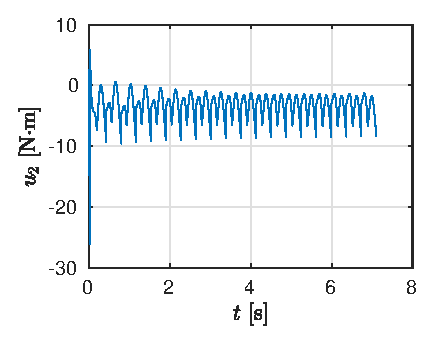
\includegraphics[width=\textwidth]{a04_control_torques_u2_optimized}
			\caption{second actuator}
		\end{center}
	\end{subfigure}
	\caption{Command angles in function of time for both actuators.}
\end{figure}

\begin{figure}[H]
	\begin{subfigure}[h]{0.8\textwidth}
		\begin{center}
			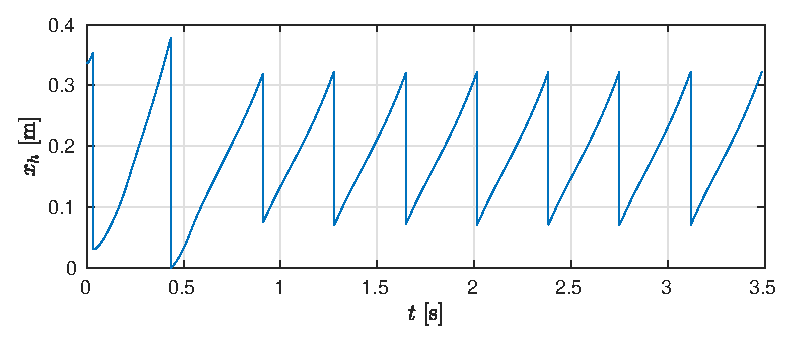
\includegraphics[width=\textwidth]{a04_x_h}
			\caption{horizontal position of the hip}
		\end{center}
	\end{subfigure}
	\begin{subfigure}[h]{0.8\textwidth}
		\begin{center}
			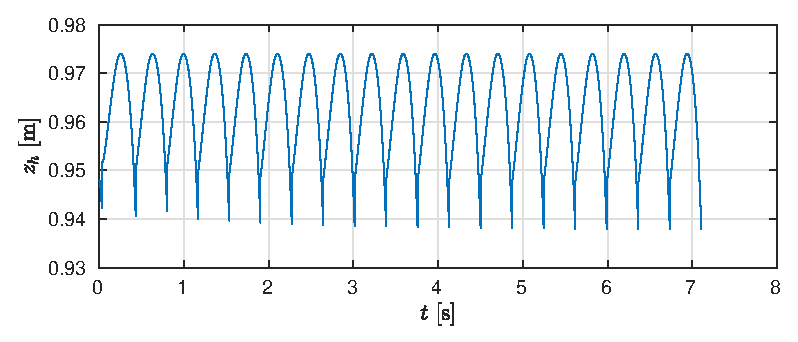
\includegraphics[width=\textwidth]{a04_z_h}
			\caption{vertical position of the hip}
		\end{center}
	\end{subfigure}
	\caption{Position of the hip as a function of time.}
\end{figure}

\begin{figure}[H]
	\begin{subfigure}[h]{0.495\textwidth}
		\begin{center}
			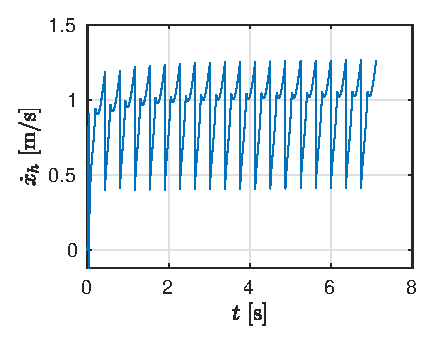
\includegraphics[width=\textwidth]{a04_dx_h}
			\caption{velocity of the hip}
		\end{center}
	\end{subfigure}
	\begin{subfigure}[h]{0.495\textwidth}
		\begin{center}
			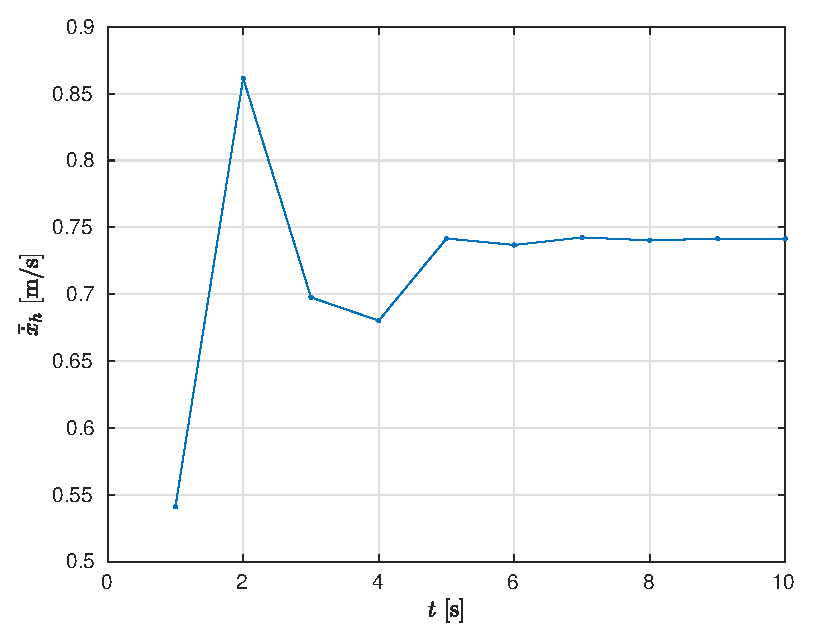
\includegraphics[width=\textwidth]{a04_average_dx_h}
			\caption{velocity of the hip averaged over the steps}
		\end{center}
	\end{subfigure}
	\caption{Velocity  of the hip in function of time / steps.}
\end{figure}

\begin{figure}[H]
	\begin{subfigure}[h]{0.495\textwidth}
		\begin{center}
			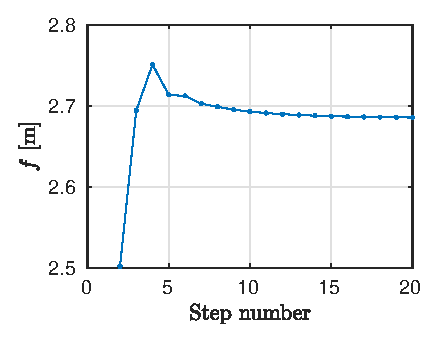
\includegraphics[width=\textwidth]{a04_step_frequency}
			\caption{step frequency}
		\end{center}
	\end{subfigure}
	\begin{subfigure}[h]{0.495\textwidth}
		\begin{center}
			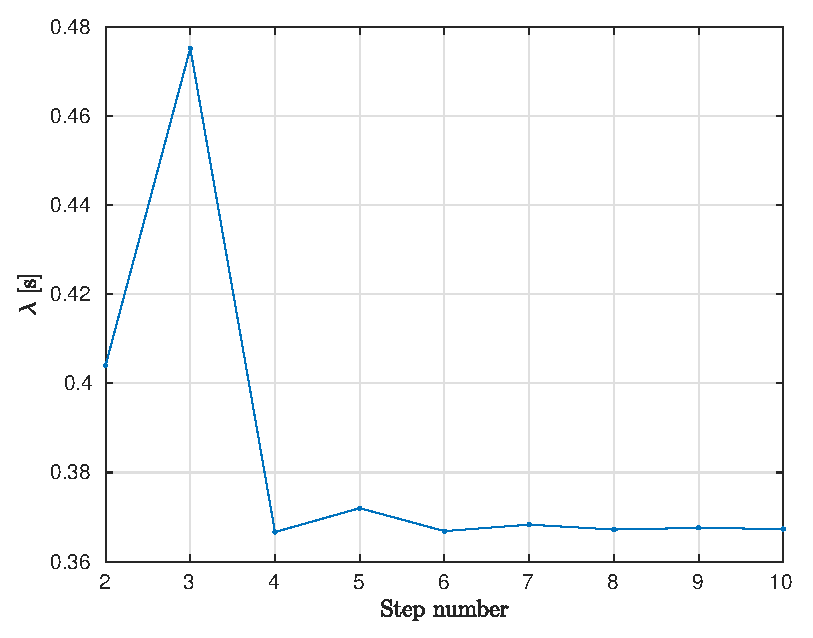
\includegraphics[width=\textwidth]{a04_step_lambda}
			\caption{step duration}
		\end{center}
	\end{subfigure}
	\caption{Regularity of the stepping.}
\end{figure}

%This gives us when computed a higher maximum and minimum velocity for the hip and swing foot. Furthermore, the input for $u_1$ and $u_2$ are also higher, while the angles for the three components of $q$ are smaller. This lead to a lower distance walked by the model over 9 steps, compared to the initial parameters. The nine steps are achieved faster but at the cost of smaller steps. The different metrics can be found here and are to be compared with those of the initial parameters when using the \verb|run\simulation.m| script.
%
%\begin{figure}[H]
%	\centering
%	\includegraphics[width=0.8\textwidth]{optimal/angle_velocity_vs_angle}
%	\caption{The angle velocity along the angle.}
%\end{figure}
%
%The maps appear to be more stable.
%
%\begin{figure}[H]
%	\centering
%	\includegraphics[width=0.8\textwidth]{optimal/angle_vs_time.png}
%	\caption{The angle of each component of $q$ throughout the simulation.}
%\end{figure}
%
%\begin{figure}[H]
%	\centering
%	\includegraphics[width=0.99\textwidth]{optimal/displacement_vs_step_number}
%	\caption{The displacement of the simulation over each steps.}
%\end{figure}
%
%\begin{figure}[H]
%	\centering
%	\includegraphics[width=0.99\textwidth]{optimal/speed_vs_time}
%	\caption{The angle velocity along the angle.}
%\end{figure}
%
%The maps appear to be more stable.
%
%\begin{figure}[H]
%	\centering
%	\includegraphics[width=0.99\textwidth]{optimal/torque_vs_time}
%	\caption{The controller input over time during the simulation}
%\end{figure}

\subsection{Reinforcment learning controller}

Because of problem of implementation, the RL controller was not completed, and thus didn't yield results.

\subsection{Virtual model controller}

	\newpage
\section{Discussions}

\subsection{Virtual constraints controller}

The goal of the assignments concerning the virtual constraints controller were met.
A functional bipedal robot was conceived following the instructions and the discussed parameters were optimized upon in order to produce a appropriate gait.
The gait has been examined both qualitatively, through the animated simulation; and quantitatively, which assessed the quality of the gait.
The steady-state was reached rather quickly, and exhibit a periodic behaviour.

\vspace{\baselineskip}

The advantages of this method is the ease of implementation of the model.
The physics are reduced to their minimum, and the hybrid model used to combine the motion of the swing foot as well as handling the stance foot proved to be reliable during the simulations.
The under actuation of the robot was handled well by the chosen controller.

\vspace{\baselineskip}

However the simplicity of this model is also its limitation.
Having the stance foot fixed on the ground while the swing foot passes through hinder the utility of this model in more realistic environment.
Numerous hypothesis to establish the gaits' equations were posed, such as an instantaneous impact of the foot, ground reaction forces and friction of the feet are not evaluated at all and the foot can't slip. 

\subsection{Reinforcement learning controller}

Reinforcement learning, had it worked, would have provided a robust simulation were the controller could have chosen from a an optimal policy the best action to take depending on the state of the robot.

\vspace{\baselineskip}

The downside to this method is the time it takes to train an agent for a problem as well as tuning the reward function effectively.
In fact the agent is sensitive to the weights and the objectives defined by the rewards, thus making this method potentially long to correctly train.
However it is most helpful when the physics of the model robot are unknown or too complicated to mathematically transcribe.
Furthermore, with a bit of knowledge on the system at hand, it is possible to guide the training of the agent, thus making it more efficient and accelerating the training phase.

\subsection{Virtual model controller}

By simulating virtual mechanical devices to induce a torque on the simulated robot just as a real mechanical device would, it is possible to control the simulated robot along a desired trajectory with precision.
Thus complex tasks are made easier by using virtual forces.
In theory virtual model control is supposed to easy to compute and and can be changed by a higher level controller during state transitions, thus guaranteeing smooth motions.

\vspace{\baselineskip}

In our case, a walking gait under actuator saturation for at least 100 steps was achieved.
The gait was maybe not what we expected, but it was a walking gait nonetheless.
The controller is robust to both internal and external perturbations, to quite an extent for external perturbations.
The optimization was very painful, and much more often than not, didn't converge to a suitable solution.
While this issue might be attributed to a badly designed controller, similar observations were made during experiments~\cite{pratt}.

\subsection{Comparison between virtual constraints and virtual model}

The virtual constraints controller's gait is much more "appropriate" than the virtual model controller.
At the very least, it is obvious when looking at the animated simulation that most scientists would emit strong reserves if such a controller (the virtual model one) were to be applied to real, physical bipedal robot.

\vspace{\baselineskip}

The normalized effort is 1.7 times bigger for the virtual model controller, but the CMT is 2.5 times bigger for the virtual constraints model.
The CMT was computed accorded to the provided expression in assignment 4.
At any rate, those two metrics were considered with caution, because they don't seem very consisten with each other, nor with other more descriptive metrics.
Typically, we would have expected the virtual model controller's CMT to be higher than the one from the virtual constraints controller.



	\section{Conclusion}

While the objective of creating a robust controller for a bipedal robot was not fully completed, this mini-project allowed us to explore a variety of controller and yielded a few results when not accounting for the saturation of the motor.
Further experimentation would be needed to achieve robust control, capable of withstanding internal and external perturbations. Furthermore, a combination of Reinforcement Learning and virtual model control could be explored, as both can be used together to achieve control of a robot executing various tasks depending on the situation.


	%%%%%%%%%%%%%%%
	%% BIBLIOGRAPHY
	%%%%%%%%%%%%%%%
	\newpage
	\section*{Bibliography} % to add a section-like unnumbered title
	\addcontentsline{toc}{section}{Bibliography} % to add said title to the toc
	\markboth{Bibliography}{Bibliography} % to modify the header
%	\printbibliography[
%	heading=subbibintoc,
%	type=article,
%	title={Articles}
%	]
	\printbibliography[
	heading=subbibintoc,
	type=thesis,
	title={Thesis}
	]
	
\end{document}
